% !TEX root = ../main.tex

\chapter{基于对抗生成网络的时间序列插值异常检测}[Cite reference]

\section{引言}[Introduction]

多变量时间序列通常含有大量的缺失值,这阻碍了高级分析方法在多变量时间序列数据中的应用。
解决缺失值的挑战的传统方法,包括均值/零插补,案例删除和基于矩阵分解的插补,都不能对多变量时间序列中的时间依赖性和复杂分布的性质进行建模。
本文将缺失值填补问题作为数据生成问题来处理。
受生成对抗网络(GAN)在图像生成方面的成功启发,本章提出用 GAN 学习多变量时间序列数据集的总体分布,进一步用于生成每个样本的缺失值。
与图像数据不同,时间序列数据由于其记录过程的性质,往往是不完整的。
GIAD 采用改进的门回归单元对不完全时间序列的时间不规则性进行建模。
在两个多变量时间序列数据集上的实验表明,该模型在缺失值场景下异常检测精度方面优于基线。

本章的组织结构如下:
3.2 节介绍融合句法信息和情感信息的文本讽刺检 测方法的总体框架以及设计细节;
3.3 节介绍本章实验部分所使用的时间序列据集以及实验设置与结果分析等;
3.4 为本章小结。

\section{基于对抗生成网络的时间序列插值异常检测}
\begin{figure}[ht]
    \label{first-model-overview}
    \centering
    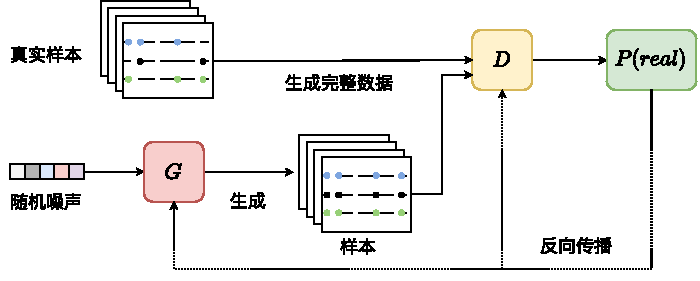
\includegraphics[width = 1\textwidth]{chapter5/overview.pdf}
    \caption{本章模型总体架构图}
    \end{figure}
图~\ref{first-model-overviw}~展示了本章方法的总体架构, 其主要包括以下几个部分: 

\textbf{面向缺失值时间序列的插值门控单元模块}:考虑到缺失值时间序列数据集存在“none”值的存在,两个连续有效观测值之间的时滞总是不断变化的。GRUI模块
通过对传统的GRU模块进行修改,引入了两个连续有效观测值的时滞变量,以保证过去观测结果的影响随着时间而衰减。

\textbf{生成器模块}:生成器模块输入一个随机噪声向量来生成一个假样本,在训练过程中通过损失函数训练生成生成的假样本接近真实样本。

\textbf{判别器模块}:判别器模块输入真实样本与生成器生成的假样本,以真假样本的差异作为损失对模型进行训练。

具体来讲,给定一组具有 $d$ 维的多变量时间序列,在 $\boldsymbol{T}=\left(t_0, \ldots, t_{n-1}\right)$中观察到的一个时间序列  $\boldsymbol{X}$ 表示为 ${X}=\left(\boldsymbol{x}_{t_0}, \ldots, \boldsymbol{x}_{t_i}, \ldots, \boldsymbol{x}_{t_{n-1}}\right)^{\top} \in \mathbb{R}^{n \times d}$, 其中 $x_{t_i}^j$  是 $\boldsymbol{x}_{t_i}$的第 $t_i$ 次观察, $x_{t_i}^j$是 $\boldsymbol{x}_{t_i}$ 的第 $j$  变量。在下面的示例中,$d=4, n=3$和 “None”缺少值。
\begin{equation}
    \boldsymbol{X}=\left[\begin{array}{cccc}
    1 & 6 & \text { none } & 9 \\
    7 & \text { none } & 7 & \text { none } \\
    9 & \text { none } & \text { none } & 79
    \end{array}\right], T=\left[\begin{array}{c}
    0 \\
    5 \\
    13
    \end{array}\right]
    \end{equation}
% The time series $\boldsymbol{X}$ is incomplete, we introduce the mask matrix $\boldsymbol{M} \in \mathbb{R}^{n \times d}$ to present whether the values of $\boldsymbol{X}$ exist or not, i.e., $M_{t_i}^j=1$, if $x_{t_i}^j$ exists, otherwise $M_{t_i}^j=0$.
时间序列 $\boldsymbol{X}$  是不完全的,本章引入掩模矩阵 $\boldsymbol{M} \in \mathbb{R}^{n \times d}$ 来表示 $\boldsymbol{X}$  的值是否存在,即,如果 $M_{t_i}^j=1$, 则$x_{t_i}^j$存在,否则 $M_{t_i}^j=0$。

为了将时间序列数据中缺失的值替换为合理的值,首先训练一个基于 GAN 的模型来学习原始时间序列数据集的分布。在这个自定义 GAN 模型中,从随机输入向量生成假时间序列的生成器和区分假数据和真数据的鉴别器将达到均衡,不仅增加了生成器的代表性能力,而且提高了鉴别器的识别能力(见图3)。其次,确定网络结构,优化生成器的输入随机向量,使生成的假时间序列能够最好地替换缺失值。

\subsection{面向缺失值时间序列的插值门控单元模块}
\begin{figure}[ht]
    \centering
    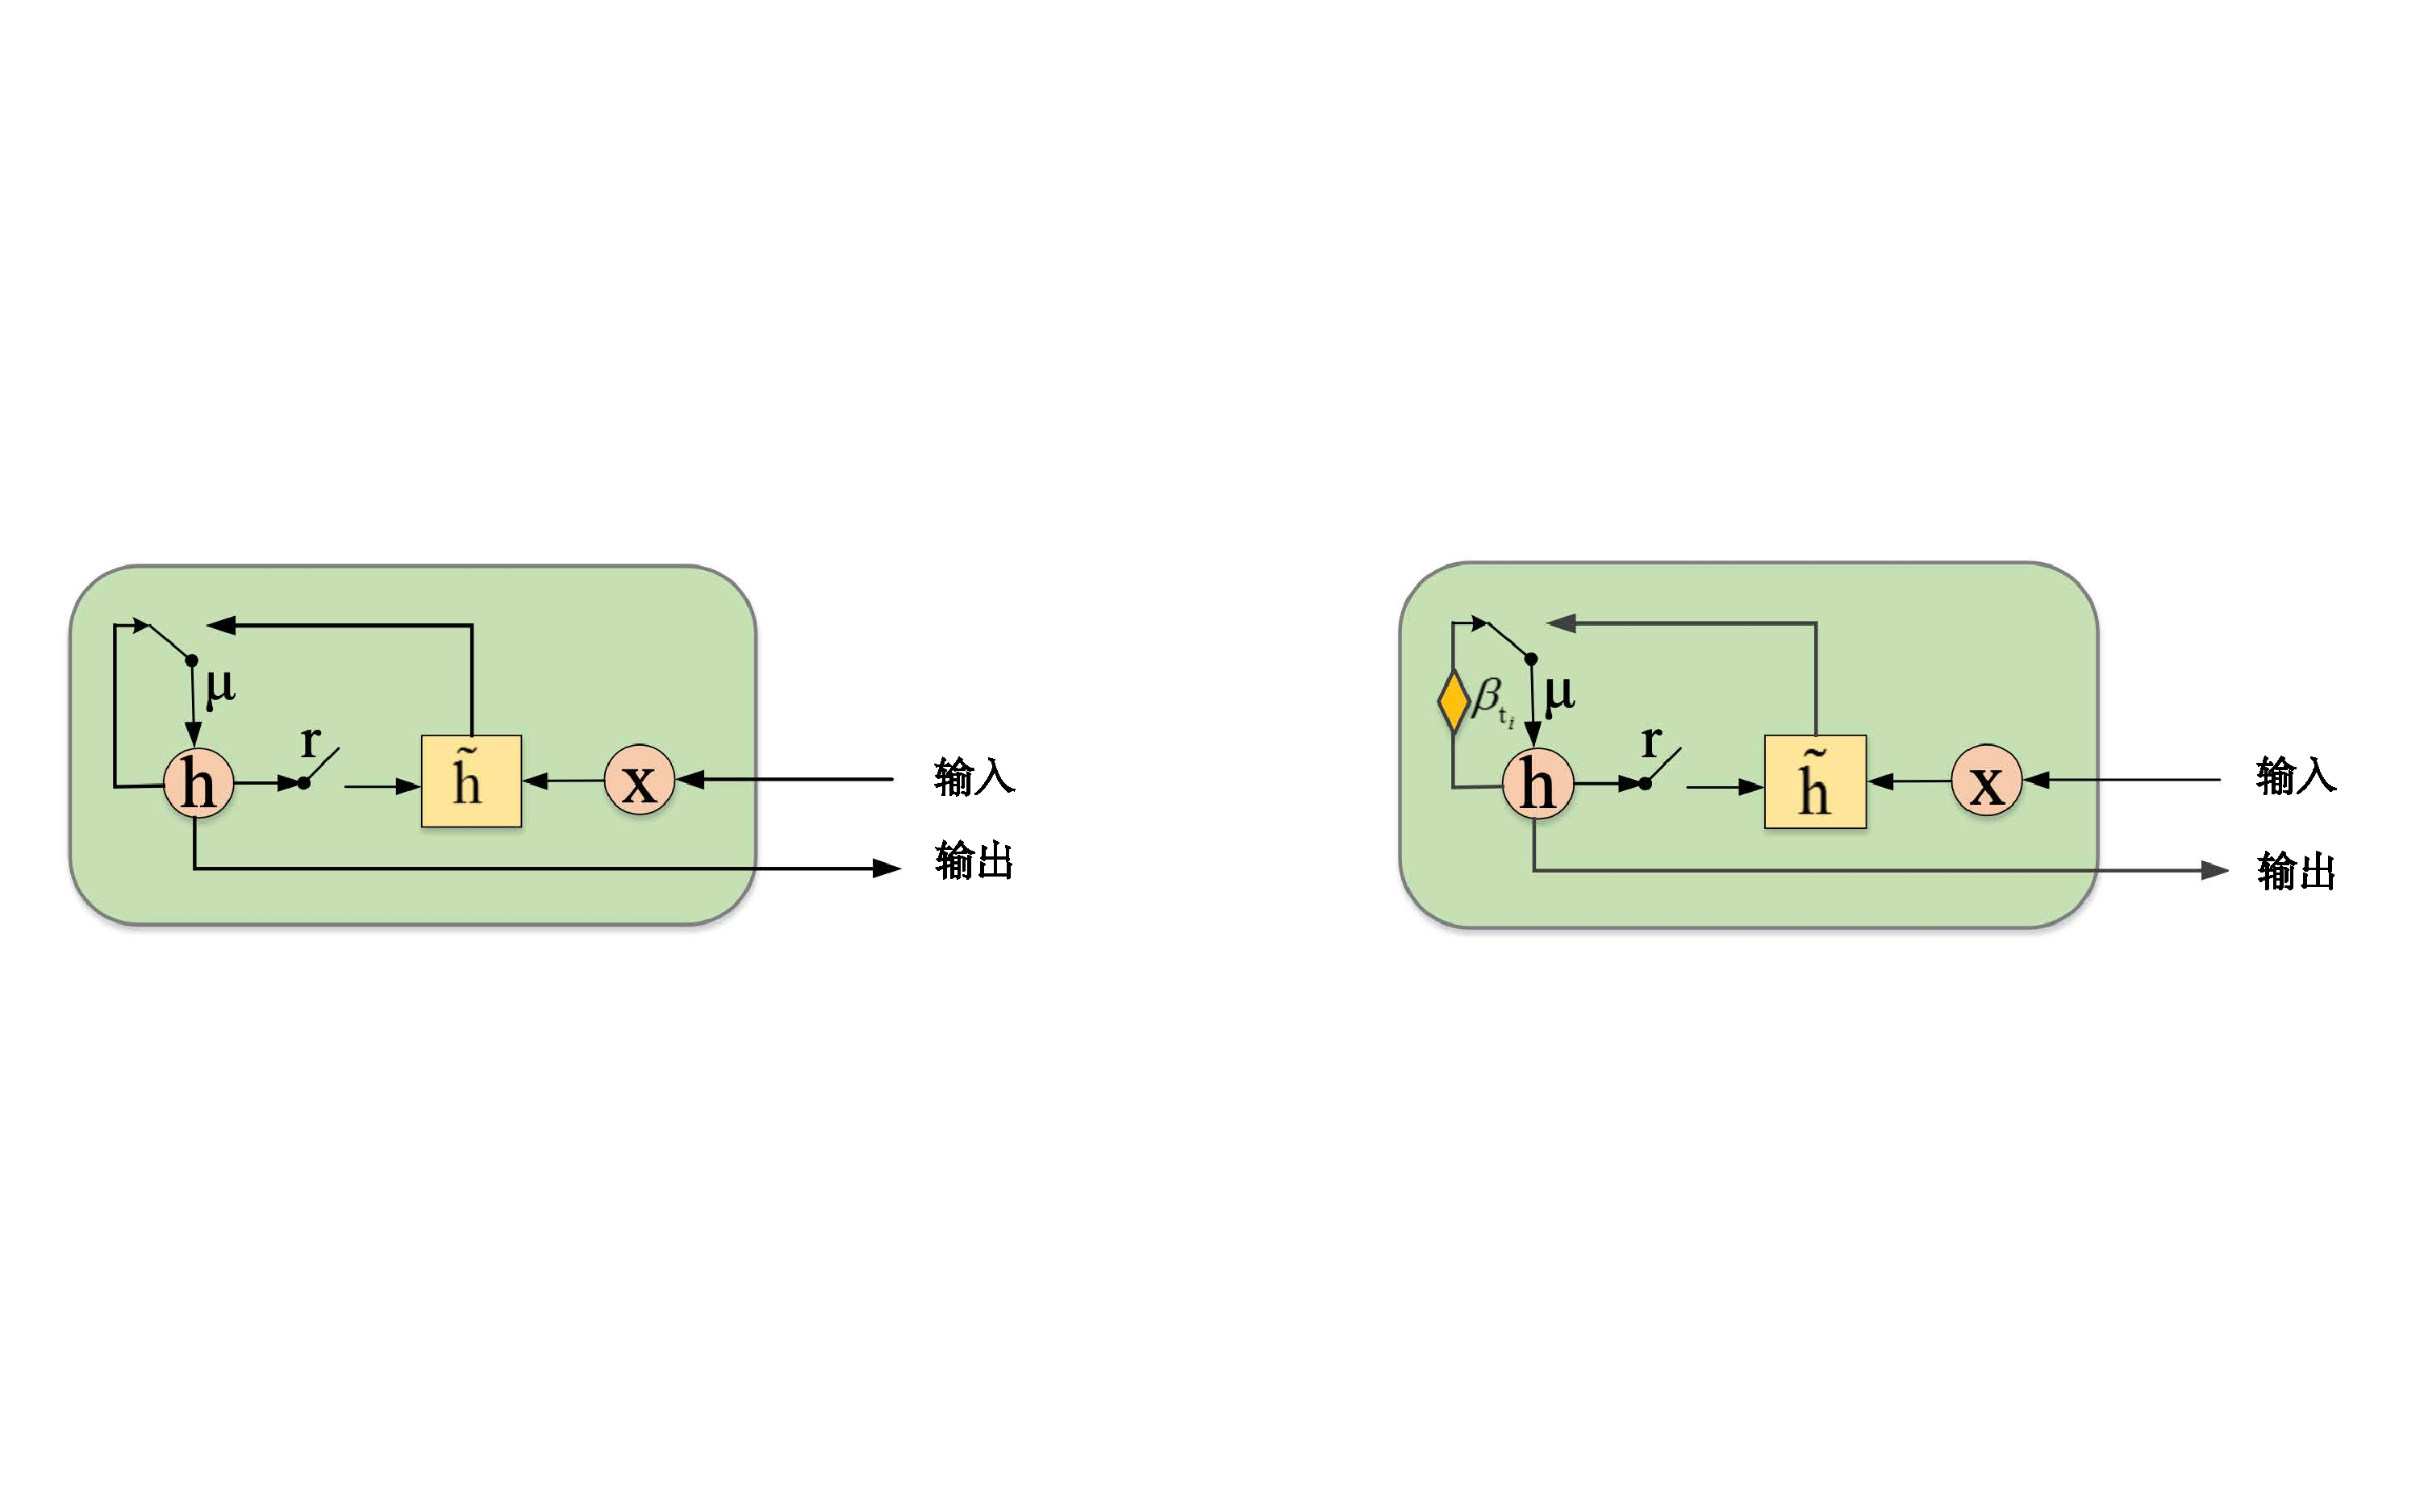
\includegraphics[width = 1\textwidth]{chapter5/GRUI.pdf}
    \caption{本章模型总体架构图}
    \end{figure}
为了适当地了解原始不完全时间序列数据集的分布和特征,并且由于“None”值的存在,两个连续有效观测值之间的时滞总是不断变化的。观测值之间的时滞非常重要,因为它们遵循未知的非均匀分布。这些可变的时间滞后提醒我们,如果变量已经丢失了一段时间,那么过去的观测结果的影响应该随着时间而衰减。为了适应这种衰减的影响,本章提出了门控递归单元的数据插补(GRUI)细胞模型的不完全时间序列的时间不规则性。

% In order to record the time lag of two adjacent existent values of $\boldsymbol{X}$, we introduce the time lag matrix $\boldsymbol{\delta} \in \mathbb{R}^{n \times d}$ to record the time lag between current value and last valid value. The followings is the calculation way and calculated results of $\delta$ of the sample dataset.
为了记录 $\boldsymbol{X}$ 的两个相邻存在值的时滞,引入时滞矩阵$\boldsymbol{\delta} \in \mathbb{R}^{n \times d}$ 来记录当前值与最后一个有效值之间的时滞。下面是样本数据集 $\delta$ 的计算方法和计算结果。
\begin{equation}
    \delta_{t_i}^j=\left\{\begin{array}{ll}
    t_i-t_{i-1}, & M_{t_{i-1}}^j==1 \\
    \delta_{t_{i-1}}^j+t_i-t_{i-1}, & M_{t_{i-1}}^j==0 \& i>0 \\
    0, & i==0
    \end{array} \quad ; \quad \boldsymbol{\delta}=\left[\begin{array}{cccc}
    0 & 0 & 0 & 0 \\
    5 & 5 & 5 & 5 \\
    8 & 13 & 8 & 13
    \end{array}\right]\right.
    \end{equation}
% We introduce a time decay vector $\boldsymbol{\beta}$ to control the influence of the past observations. Each value of the $\boldsymbol{\beta}$ should be bigger than zero and smaller than one, and the larger the $\boldsymbol{\delta}$, the smaller the decay vector.
% So we model the time decay vector $\boldsymbol{\beta}$ as a combination of $\boldsymbol{\delta}$ :
本模型引入一个时间衰减向量 $\boldsymbol{\beta}$ 来控制过去观测的影响。$\boldsymbol{\beta}$ 的每个值应大于0,小于1,$\boldsymbol{\beta}$  越大,衰减矢量越小。
因此,本模型将时间衰减向量 $\boldsymbol{\beta}$  模拟为 $\boldsymbol{\delta}$ 的组合:   
\begin{equation}
    \boldsymbol{\beta}_{t_i}=1 / e^{\max \left(\mathbf{0}, \boldsymbol{W}_\beta \delta_{t_i}+\boldsymbol{b}_\beta\right)},
    \end{equation}
% where $\boldsymbol{W}_\beta$ and $\boldsymbol{b}_\beta$ are parameters that need to learn. We use the negative exponential formulation to 
% make sure that $\boldsymbol{\beta}_{t_i} \in(\mathbf{0}, \mathbf{1}]$. Besides, in order to capture the interactions of the $\delta$ 's variables, 
% we prefer full weight matrix to diagonal matrix for $\boldsymbol{W}_\beta$. After we have got the decay vector, we update the GRU hidden state 
% $\boldsymbol{h}_{t_{i-1}}$ by element-wise multiplying the decay factor $\boldsymbol{\beta}$. Since we have used the batch normalization [24] 
% technology, the hidden state $\boldsymbol{h}$ is smaller than 1 with a high probability.We choose multiplicative decay way rather than some 
% other decay ways such as $\boldsymbol{h}^{\boldsymbol{\beta}}$. The update functions of GRUI are:
$\boldsymbol{W}_\beta$ 和 $\boldsymbol{b}_\beta$ 是需要学习的参数。利用负指数形式确定 $\boldsymbol{\beta}_{t_i} \in(\mathbf{0}, \mathbf{1}]$。
此外,为了捕捉 $\delta$ 变量之间的相互作用,对于 $\boldsymbol{W}_\beta$,本方法更倾向于使用全权矩阵而不是对角矩阵。
在得到衰减矢量之后,本方法用元素方法乘以衰减因子 $\boldsymbol{\beta}$ 来更新 GRU 的隐状态 $\boldsymbol{h}_{t_{i-1}}$。
由于本方法使用了批量归一化技术 ,隐状态 $\boldsymbol{h}$ 小于1的概率很高。本方法选择了乘法衰减方式,而不是其他衰减方式,如  $\boldsymbol{h}^{\boldsymbol{\beta}}$。
其次,确定网络结构,优化生成器的输入随机向量,使生成的假时间序列能够最好地替换缺失值。GRUI 的更新功能如下:    
\begin{equation}
    \boldsymbol{h}_{t_{i-1}}^{\prime}=\boldsymbol{\beta}_{t_i} \odot \boldsymbol{h}_{t_{i-1}}
    \end{equation}
\begin{equation}
    \boldsymbol{\mu}_{t_i}=\sigma\left(\boldsymbol{W}_\mu\left[\boldsymbol{h}_{t_{i-1}}^{\prime}, \boldsymbol{x}_{t_i}\right]+\boldsymbol{b}_\mu\right), \quad \boldsymbol{r}_{t_i}=\sigma\left(\boldsymbol{W}_r\left[\boldsymbol{h}_{t_{i-1}}^{\prime}, \boldsymbol{x}_{t_i}\right]+\boldsymbol{b}_r\right)
    \end{equation}
\begin{equation}
    \tilde{\boldsymbol{h}}_{t_i}=\tanh \left(\boldsymbol{W}_{\tilde{h}}\left[\boldsymbol{r}_{t_i} \odot \boldsymbol{h}_{t_{i-1}}^{\prime}, \boldsymbol{x}_{t_i}\right]+\boldsymbol{b}_{\tilde{h}}\right), \quad \boldsymbol{h}_{t_i}=\left(\mathbf{1}-\boldsymbol{\mu}_{t_i}\right) \odot \boldsymbol{h}_{t_{i-1}^{\prime}}+\boldsymbol{\mu}_{t_i} \odot \tilde{\boldsymbol{h}}_{t_i}
    \end{equation}
\begin{equation}
\tilde{\boldsymbol{h}}_{t_i}=\tanh \left(\boldsymbol{W}_{\tilde{h}}\left[\boldsymbol{r}_{t_i} \odot \boldsymbol{h}_{t_{i-1}}^{\prime}, \boldsymbol{x}_{t_i}\right]+\boldsymbol{b}_{\tilde{h}}\right), \quad \boldsymbol{h}_{t_i}=\left(\mathbf{1}-\boldsymbol{\mu}_{t_i}\right) \odot \boldsymbol{h}_{t_{i-1}^{\prime}}+\boldsymbol{\mu}_{t_i} \odot \tilde{\boldsymbol{h}}_{t_i}
\end{equation}
$\boldsymbol{\mu}$ 是更新门,$\boldsymbol{r}$ 是复位门,$\tilde{\boldsymbol{h}}$ 是候选隐状态,$\sigma$ 是 sigmoid 激活函数,$\boldsymbol{W}_{\tilde{h}}, \boldsymbol{W}_r, \boldsymbol{W}_\mu, \boldsymbol{b}_\mu, \boldsymbol{b}_r$ 
和 $\boldsymbol{b}_{\tilde{h}}$是训练参数,$\odot$ 是元素乘法。

\subsection{生成器模块和判别器模块}
判别器$D$ 首先由 GRUI 层组成,以学习不完整或完整的时间序列。然后,在 GRUI 的最后一个隐藏状态的顶部堆叠一个完全连接层。为了防止过度配合,本方法采用了在全连接层实用了Dropout。
当我们把原始的不完全实时序列输入到 $D$ 中时,$\delta$  的一行的值是不相同的。当本方法输入由 $G$ 生成的假时间序列时,$\delta$  的每一行的值都是相同的(因为没有缺失值)。
我们希望确保生成的示例的时间滞后与原始示例的时间滞后相同,因此 $\mathrm{G}$ 还由 GRUI 层和完全连接层组成。
$\mathrm{G}$ 是一个自馈网络,它意味着 $G$ 的当前输出将被反馈到同一个单元的下一次迭代中。$G$ 的第一个输入是随机噪声向量 $\boldsymbol{z}$,假样本 $\delta$  的每一行都是一个常数值。

\subsection{模型训练}
% From the GAN architecture, we can know that, the generator G can learn a mapping
% $G(\boldsymbol{z})=\boldsymbol{z} \mapsto \boldsymbol{x}$ that maps the random
% noise vector $\boldsymbol{z}$ to a complete time series which contains no
% missing value. However, the problem is the random noise vector $\boldsymbol{z}$
% is randomly sampled from a latent space, e.g., Gaussian distribution. It means
% that, the generated samples may change a lot with the changing of the input
% random noise $\boldsymbol{z}$. Although the generated samples obey the
% distribution of the original samples, the distance between the generated samples
% and the original samples may also be large. In other words, the degree of
% similarity between $\boldsymbol{x}$ and $G(\boldsymbol{z})$ is not large enough.
% For example, the original incomplete time series contains two classes, and the
% $\mathrm{G}$ learns a distribution that can fit these two classes very well.
% Given a incomplete sample $\boldsymbol{x}$ and a random input vector
% $\boldsymbol{z}$, the $G(\boldsymbol{z})$ may belong to the opposite class of
% $\boldsymbol{x}$, this is not what we want. Although the $G(\boldsymbol{z})$ may
% belong to the true class, the similarity of samples within a class could also be
% large.
通过 GAN 结构,可以知道,生成器 G 可以学习一个映射 $G(\boldsymbol{z})=\boldsymbol{z} \mapsto \boldsymbol{x}$ ,
它将随机噪声向量 $\boldsymbol{z}$ 映射到一个完整的时间序列,
该序列不包含任何缺失值。
然而,问题是随机噪声向量 $\boldsymbol{z}$ 是从一个潜在的空间中随机采样的,例如,正态分布。这意味着,随着输入随机噪声 $\boldsymbol{z}$ 的变化,
生成的样本可能发生很大的变化,虽然生成的样本服从原始样本的分布,但是生成的样本与原始样本之间的距离也可能很大。
换句话说,$\boldsymbol{x}$ 和$G(\boldsymbol{z})$之间的相似度不够大。
例如,原始的不完全时间序列包含两个类,并且 $\mathrm{G}$ 学习了一个能很好地适应这两个类的分布。
给定一个不完全样本 $\boldsymbol{x}$ 和一个随机输入向量 $G(\boldsymbol{z})$,$G(\boldsymbol{z})$ 可能属于 x 的相反类,这不是我们想要的。
虽然 $G(\boldsymbol{z})$ 可能属于真正的类,但类内样本的相似性也可能很大。

对于任何不完全的时间序列 $\boldsymbol{x}$ ,本方法试图从潜在的输入空间中找到一个最佳向量 z,$G(\boldsymbol{z})$与 $\boldsymbol{x}$ 
最相似。如何用最合理的值替换缺失的值?
受\cite{gan}的启发,本方法介绍了一种度量归责适应度的方法。本方法定义了一个两部分损失函数来评估插补的适应性。
这个损失函数的第一部分是掩蔽重建损失。这意味着生成的样本 $G(\boldsymbol{z})$应该足够接近原始的不完全时间序列 $\boldsymbol{x}$ 。
这个损失函数的另一部分是判别损失。这一部分迫使生成的样本 $G(\boldsymbol{z})$尽可能真实。以下各段将详细描述被掩盖的重建损失和歧视性损失。

\textbf{掩码重建损失}: 掩码重建损失是由原始样本 $\boldsymbol{x}$ 和生成样本 $G(\boldsymbol{z})$之间的掩模平方误差决定的。值得注意的是,本方法只计算非缺失的部分数据。
\begin{equation}
    L_r(\boldsymbol{z})=\|\boldsymbol{X} \odot \boldsymbol{M}-G(\boldsymbol{z}) \odot \boldsymbol{M}\|_2 .
    \end{equation}
\textbf{判别器损失}:判别器损失代表生成的样本 $G(\boldsymbol{z})$ 的真实性程度。它是基于判别器 $D$的输出,它表示输入样本 $G(\boldsymbol{z})$
是真实的置信水平。
本方法把噪声向量 $\boldsymbol{z}$ 输入到 $G$ 中,然后得到产生的样本 $G(\boldsymbol{z})$ ,接着把 $G(\boldsymbol{z})$ 输入到 $D$中,最后得到判别损失。
\begin{equation}
    L_d(\boldsymbol{z})=-D(G(\boldsymbol{z}))
    \end{equation}
\textbf{插补损失}:为了优化随机噪声矢量 $\boldsymbol{z}$ ,本方法定义了插补损失。假设损失是掩蔽重建损失和区分性损失的结合。
\begin{equation}
    L_{\text {imputation }}(\boldsymbol{z})=L_r(\boldsymbol{z})+\lambda L_d(\boldsymbol{z})
    \end{equation}
其中 λ 是一个超参数,控制掩蔽重建损失和判别损失之间的比例。


对于每一个原始的时间序列 $\boldsymbol{x}$ ,本方法随机抽样一个具有零均值和单位方差的正态分布,
并将其输入到训练有素的生成器 $G$ 中,以得到 $G(\boldsymbol{z})$。
然后,本方法开始训练噪声 $\boldsymbol{z}$ 与损失函数 $L_{\text {imputation }}(\boldsymbol{z})$的反向传播方法。
在插补损失收敛到最优解之后,本方法用生成的 $G(\boldsymbol{z})$代替缺失的 $\boldsymbol{x}$ 值,如下面的方程所示,
\begin{equation}
    \boldsymbol{x}_{\text {imputed }}=\boldsymbol{x} \odot \boldsymbol{M}+(\mathbf{1}-\boldsymbol{M}) \odot G(\boldsymbol{z})
    \end{equation}
%最后,我们针对$\boldsymbol{x}_{\text {imputed }}$执行

\section{实验结果与分析}

\subsection{实验数据集}
本章实验所用数据集选自NASA发布的有关卫星收集的遥测时间序列数据集SMAP和\cite{msl}。

\textbf{SMAP(Soil Moisture Active Passive satellite)}: 土壤水分主动被动卫星数据集。时间信息匿名(时间粒度是分钟),数据已全被缩放到0-1之间。SMAP有55个实体,每个实体有25个维度。
只有telemetry value是连续变量,其他变量都是相关命令(command)是否发送,实际就是0或者1(0为没发送,而1代表已发送)
训练集无标签,测试集有标签。

\textbf{MSL(Mars Science Laboratory rover)}:火星科学实验室探测车数据集。时间信息匿名(时间粒度是分钟),数据已全被缩放到0-1之间。MSL有27个实体,每个实体有25个维度。
只有telemetry value是连续变量,其他变量都是相关命令(command)是否发送,实际就是0或者1(0为没发送,而1代表已发送)
训练集无标签,测试集有标签。

训练集中皆为正常数据,测试集中存在有两种异常,point和contextual,前者点异常,后者是整体变化趋势异常。该数据集统计信息如表4-1所示:
\begin{table}[htbp]
    \caption{所有方法在SWAT数据集上的性能比较}
    \vspace{0.5em}\centering\wuhao
    \begin{tabular}{ccccc}
    \toprule
    统计信息 & SMAP & MSL & \\
    \midrule
    异常序列总数	& 69	& 36 \\
    点异常数	& 43(62\%)	& 62(59\%)\\ 
    上下文异常数	& 26(48\%)	& 43(41\%) \\
    维度	& 55	& 25\\
    观测值数量	& 429735	& 66709 \\
    \bottomrule
    \end{tabular}
    \end{table}

\subsection{实验设置}
本方法测试了不同程度下删除数据后模型性能表现。通过实验结果可以看到,本方法在SOTA模型的原场景下接近SOTA的性能,
同时在本章设计的新的场景下超过SOTA模型的表现,以此可以证明本章的模型在缺失值场景下具有较好的性能表现。
同时本章的模型在beta = 0 至 beta = 0.3 与 beta = 0.3 至 beta = 0.5 的场景变换中,性能下降最低,这证明了本章的模型在数据损失的情况下性能
下降最不明显,对数据缺失具有鲁棒性。

判别器由一个 GRUI 层和一个全连接层组成。将实不完全时间序列 $\boldsymbol{x}$、伪完全时间序列 $G(\boldsymbol{z})$及其对应的 $\delta$ 输入 GRUI 层。然后将 GRUI 层的最后一个隐藏状态以一个中断的形式输入到全连接层,以获得鉴别器的输出。生成器是一个自馈网络,由 GRUI 层和完全连接层组成。将 GRUI 层当前的隐藏状态通过一个中断输入到全连接层,然后将全连接层的输出作为下一次迭代的输入。

\subsection{模型基线说明}
\textbf{AutoEncoder}: 自编码器\cite{none1}, 是一种无监督式学习模型。它基于反向传播算法与最优化方法利用输入数据 $X$ 本身作为监督, 来指导神经网络尝试学习一个映射关系, 
从而得到一个重构输出 $X^R$ 。在时间序列异常检测场景下, 异常对于正常来说是少数, 如果使用自编码器重构出来的输出 $X^R$ 跟原始输入的差异超出一定阈值则存在异常。

\textbf{IsolationForest}: 孤立森林\cite{none2},它一般由若干个决策树构成。每棵树随机抽取特征、随机选取分割值来建立决策树,
从而将每一个样本分到一个独立的子节点上。通过估计每个样本在各个决策树上距离根节点的期望路径长度进行异常判别。

\textbf{LSTM-NDT}: Hundman等人\cite{lstm-ndt}在2018年发表在KDD上的无监督异常检测模型,提出通过LSTM对序列进行预测,将预测值与真实值进行比较,并提出一种非参数动态阈值设定方法来设定预测值
与真实值的差距,并以此判定异常。

\subsection{性能对比及分析}

% 表4-2中分别列举了所有基线模型以及本章方法在 Twitter-Cai 数据集中的性 能表现。 对于 ResNet、ViT 等图像单模态模型,
% 本章实验仅使用图像模态输入对其进行训练。对于TextCNN、SIARN 等文本单模态模型,本章实验仅使用文本模态输入对其进行训练。
% 对于 HFM、D\&RNet 等图文多模态模型以及本章方法,本章实验使用文本和图像模态输入对其进行训练。
% 为了更加公平的比较,对 于 HFM、D\&R Net 等文章中使用与本文相同数据集和数据划分的模型,本章实 验部分摘抄其文章内的性能统计结果。
% 对于 ResNet、TextCNN 等通用模型以及 SIARN 等文本讽刺检测模型,本章实验使用其在相同数据集和数据划分中不同 随机种子训练 10 次的平均性能作为统计结果。
% 从实验结果中可以看到,在全部 7 种评价指标上,本章方法都能显著超过 所有基线模型,达到最优效果。具体来讲,本章方法准确率超过第二名的基线模型 1.5\%, 精确率、召回率和 
% F1 值分别超过第二名的基线模型 4.91\%、0.54\% 和 3.26\%。在 Macro
% 平均后的统计指标上,本章方法精确率、召回率和 F1 值分 别超过第二名的基线模型 5.71\%、1.89\% 和 4.08\%。总体来说,本章的方法在图
% 文多模态讽刺检测任务中显著超越已有的基线模型, 取得了最优性能。
本章实验主要在两个数据集上对比三个对比方法进行实验。由于使用的数据集都是完整不包含缺失值的数据,为了能够比较在缺失值场景下模型的性能,
设定了两个缺失值场景,即缺失率为30\%和缺失率为50\%。为了模拟缺失值,在进行实验前对数据进行数据进行缺失预处理,程序对原有数据集随机删除30\%50\%的数据。
由于AutoEncoder,IsolationForest,LSTM-NDT不允许数据中存在“None”值,故删除的数据以-1代替。为消除随机性带来的误差,以下实验结果均为5次平均后的结果。

实验结果表明,本章提出的基于对抗生成网络的多元时间序列插值异常检测模型在多个场景均超过了基线方法。
具体来讲,在完整数据集上,本章F1分数超过了第二名的基线0.3\%
在缺失30\%数据的场景下F1分数超过了第二名的基线3\%,在缺失50\%数据的场景下F1分数超过了第二名的基线5\%。证明了本章的算法在缺失值场景的有效性。

\begin{table}[htp]
    \caption{所有方法在SMAP数据集上的性能比较}
    %\label{comparison_results}
    \small
    \centering
    \setlength{\tabcolsep}{0.8mm}{
    \begin{tabular}{lccccccccc}\toprule
    Method & \multicolumn{3}{c}{SMAP 完整数据集} & \multicolumn{3}{c}{SMAP 删除30\%数据} & \multicolumn{3}{c}{SMAP 删除50\%数据} \\ \cmidrule(r){2-4} \cmidrule(r){5-7} \cmidrule(r){8-10}
        & Precision & Recall & F1分数 & Precision & Recall & F1分数& Precision & Recall & F1分数\\ \midrule
        AE & 0.721	& 0.979	& 0.77	& 0.576	& 0.783	& 0.664	& 0.461	& 0.626	& 0.531\\ 
        IF	& 0.442	& 0.51	& 0.46	& 0.353	& 0.408	& 0.378	& 0.282	& 0.326	& 0.303\\ 
        LSTM-NDT	& 0.855	& 0.61	& 0.71	& 0.684	& 0.488	& 0.569	& 0.547	& 0.39	& 0.455\\ 
        GIAD	& 0.844	& 0.79	& \textbf{0.816}	& 0.717& 	0.671	& \textbf{0.693}& 	0.609& 	0.52	& \textbf{0.561}\\ 
  %\bfseries MUSE-Net& \bfseries 2.89 & \bfseries 1.10 & \bfseries 2.74 & \bfseries 1.05 & \bfseries 15.47 & \bfseries 5.47 & \bfseries 14.45 & \bfseries 5.54 & \bfseries 17.19 \\
  \bottomrule
  \centering
  \end{tabular}}
  \end{table}

  \begin{table}[htp]
    \caption{所有方法在MSL数据集上的性能比较}
    %\label{comparison_results}
    \small
    \centering
    \setlength{\tabcolsep}{0.8mm}{
    \begin{tabular}{lccccccccc}\toprule
    Method & \multicolumn{3}{c}{MSL 完整数据集} & \multicolumn{3}{c}{MSL 删除30\%数据} & \multicolumn{3}{c}{MSL 删除50\%数据} \\ \cmidrule(r){2-4} \cmidrule(r){5-7} \cmidrule(r){8-10}
        & Precision & Recall & F1分数 & Precision & Recall & F1分数& Precision & Recall & F1分数\\ \midrule
        AE	& 0.853	& 0.974	& 0.879& 	0.682	& 0.779	& 0.727& 0.545& 	0.623& 	0.582\\
        IF	& 0.568	& 0.674	& 0.598	& 0.454	& 0.539	& 0.493	& 0.363	& 0.431	& 0.39\\
        LSTM-NDT	& 0.926	& 0.694	& 0.69	& 0.74	& 0.555	& 0.634	& 0.592	& 0.444	& 0.507\\
        GIAD	& 0.866	& 0.894	& \textbf{0.88}	& 0.736	& 0.759	& \textbf{0.747}	& 0.625	& 0.645	& \textbf{0.635}\\
  %\bfseries MUSE-Net& \bfseries 2.89 & \bfseries 1.10 & \bfseries 2.74 & \bfseries 1.05 & \bfseries 15.47 & \bfseries 5.47 & \bfseries 14.45 & \bfseries 5.54 & \bfseries 17.19 \\
  \bottomrule
  \centering
  \end{tabular}}
  \end{table}

\section{本章小节}
本章介绍了基于对抗生成网络的时间序列插值异常检测方法。
通过对当前缺失值多元时间序列异常检测场景的分析,本章提出了一种基于插值补全的多元时间序列异常检测算法。
通过与多个基线模型对比,在完整数据集上,本章F1分数超过了第二名的基线0.3\%
在缺失30\%数据的场景下F1分数超过了第二名的基线3\%,在缺失50\%数据的场景下F1分数超过了第二名的基线5\%。
证明了本章算法在缺失值场景的有效性。

